%----------------------------------------------------------------------------------
%% MCM/ICM LaTeX Template %%
%% 2024 MCM/ICM           %%
%----------------------------------------------------------------------------------
%不超过25面(包括任何内容)
%字体不小于12号
%摘要十分重要!!!
%如果使用AI工具,就需要在AI使用报告中说明,不计入25面中

\documentclass[UTF8]{ctexart} % 文档类型,中文
\usepackage{fontspec} % 字体设置
\usepackage{geometry} % 页面设置
\usepackage{setspace} % 行间距
\usepackage{amsmath,amssymb,amsthm} % 公式
\usepackage{unicode-math} % 公式(一些特殊符号)
\usepackage{tabularx} % 表格
\usepackage{booktabs} % 表格线
\usepackage{multirow} % 多行合并
\usepackage{graphicx} % 图片
\usepackage{float}  % 图片位置控制(htpd,H)
\usepackage{caption} % 图片标题
\usepackage{fancyhdr} % 页眉页脚
\usepackage{listings} % 代码
\usepackage{xcolor} % 代码颜色高亮
\usepackage{url} % 引用链接
\usepackage{appendix} % 附录
\usepackage{hyperref} % 超链接
\usepackage[english]{babel}

\newcommand{\Problem}{C} % 哪一题,在这里修改
\newcommand{\Team}{2416996} % 队伍编号,在这里修改

\addto\captionsenglish{
  \renewcommand{\figurename}{Fig.} % 图片标题
  \renewcommand{\tablename}{Table} % 表格标题
}

\setmainfont{Times New Roman}  % 将主字体设置为 Arial/Times new roman
\geometry{a4paper,scale=0.8,headheight=15pt} % 页面设置,A4纸,缩放0.8
\setstretch{1.5} % 行间距1.5倍
\setmathfont{Latin Modern Math} % 公式字体
\captionsetup[table]{belowskip=10pt} % 表格标题与表格距离
\hypersetup{
    colorlinks=true,
    linkcolor=black,
    citecolor=black,
    urlcolor=black
} % 超链接颜色

\pagestyle{fancy} % 页眉页脚
\lhead{Team \# \Team}
\rhead{Page \thepage\ of 25} % 注意修改总页数
\cfoot{\empty}
\renewcommand{\headrulewidth}{0.4pt} % 页眉线宽度

% 定义代码高亮部分的颜色(随便调的,可改)
\definecolor{codepink}{RGB}{255, 183, 255}
\definecolor{codePink}{RGB}{255, 60, 255}
\definecolor{codepurple}{RGB}{204, 0, 204}
\definecolor{codeYellow}{RGB}{255, 255, 179}
\definecolor{codeyellow}{RGB}{248, 242, 25}
\definecolor{codeGreen}{RGB}{60, 200, 160}
\definecolor{codegreen}{RGB}{142, 255, 29}
\definecolor{codeBlue}{RGB}{0, 151, 254}
\definecolor{codeblue}{RGB}{133, 235, 255}
\definecolor{codegray}{RGB}{234, 234, 234}
\definecolor{codered}{RGB}{255, 102, 153}
\definecolor{backcolour}{RGB}{242, 242, 235}

% 代码高亮部分的样式设置
\lstdefinestyle{mystyle}{
    backgroundcolor=\color{white},      % 代码块背景色  
    basicstyle=\small,                  % 代码块字体大小(\tiny\scriptsize\footnotesize\small\normalsize\large\Large\LARGE\huge\Huge)
    frame=single,                       % 代码之外显示边框 (none/leftline/topline/bottomline/lines/single/shadowbox)
    framesep=0pt,                       % 设置上下边框与代码块内容的距离
    xleftmargin=0pt,                    % 代码块左侧空白
    xrightmargin=0pt,                   % 代码块右侧空白
    breakindent=75pt,                   % 设置换行后的行的缩进
    rulecolor=\color{black},            % 指定边框的颜色
    commentstyle=\color{codeGreen},     % 注释风格颜色
    keywordstyle=\color{codePink},      % 关键字风格颜色 可以规定关键字为keywords={if, end...}
    stringstyle=\color{codeBlue},       % 字符串风格颜色
    numberstyle=\color{codered},        % 行号风格颜色
    numbers=left,                       % 行号位置为左侧(left\right\none)
    numbersep=5pt,                      % 行号与代码块距离 
    breakatwhitespace=false,            % 是否在空格处换行
    breaklines=true,                    % 是否自动换行
    % prebreak=\raisebox{0ex}[0ex][0ex]{\ensuremath{\hookleftarrow}},  % 换行符号
    keepspaces=true,                    % 是否保留空格
    showspaces=false,                   % 是否强调空格
    showstringspaces=false,             % 是否强调代码中的字符串
    showtabs=false,                     % 是否强调制表符
    tabsize=2,                          % 设置制表符长度为2个字符
    % escapeinside={*},                 % 特定的字符,退出源码模式到LaTeX模式 (例如 escapeinside={\%*}{*)})
    captionpos=b,                       % 设置标题位置为底部(t\b)
}
\lstset{style=mystyle}

\begin{document}

\thispagestyle{empty} % 首页无页眉页脚
\vspace*{-12ex}
\centerline{\begin{tabular}{*3{c}}
	\parbox[t]{0.3\linewidth}{\begin{center}\textbf{Problem Chosen}\\ \Large {\Problem}\end{center}}
	& \parbox[t]{0.3\linewidth}{\begin{center}\textbf{2024\\ MCM/ICM\\ Summary Sheet}\end{center}}
	& \parbox[t]{0.3\linewidth}{\begin{center}\textbf{Team Control Number}\\ \Large {\Team}\end{center}}	\\
	\hline
\end{tabular}}

\vspace*{5ex}
{\centering \Large \textbf{Momentum and Turning Points Prediction in Tennis Games} \par}

%Summary Sheet
%----------------------------------------------------------------------------------
{\centering \Large \textbf{Summary} \par}
Firstly, we represented the player's current performance performance by summing the scores of their recent ten points, reflecting the game situation. 
Through a correlation matrix, we identified strong correlations between the current performance performance and variables like the serving side, score difference, recent lethal shots, error count, 
and break point count, indicating a significant connection between player performance and game performance.

Next, logistic regression was applied to predict the occurrence of turning points, using selected strongly correlated factors as variables. After defining turning points as observations, 
we achieved high accuracy in logistic regression on all data. Thus, we used the obtained weights and intercept to establish a linear combination of these variables as the player's momentum. 
We then conducted a correlation analysis between turning points and these variables, identifying influential factors such as the recent five-point scores of p1 and p2, 
the current serving side, and recent successful breaks by p1 and p2.

Following that, we demonstrated in two ways that the turning points in the matches are not random. Firstly, we identified actual turning points in a game, 
subjected them to a run test, and found that their occurrence is not random. Secondly, we used the model to predict turning points and assessed the overlap between predicted and actual turning points using Pearson Correlation and Jaccard similarity, 
revealing a high degree of concordance. This demonstrated that actual turning points are significantly related to current game data and momentum, rather than occurring randomly.

Subsequently, we trained the model with specific player game data, obtained a particular function for the player's momentum, and analyzed the weights. 
We identified the significant factors influencing this player and formulated strategies tailored to the player's strengths and weaknesses. 
Applying the previously derived turning point prediction formula to five matches in Wimbledon, we used the Jaccard test to assess their similarity. 
The results indicated a high degree of similarity between the predicted and actual sets. But the similarity in some matches was not very high, 
which could be attributed to the oversight of certain match factors, such as differences in skill levels between players and variations in the duration of the matches.

\noindent \textbf{Keywords:} tennis, momentum, turning points, logistic regression, prediction 
%----------------------------------------------------------------------------------


% contents 记得更新页面或者用section指令
%----------------------------------------------------------------------------------
\newpage
\tableofcontents
\newpage
%----------------------------------------------------------------------------------


% Introduction 下面列举了四个小部分,可包含两到三个
%----------------------------------------------------------------------------------
\section{\textbf{Introduction}}
\subsection{\textbf{Problem Background}}
In the 2023 Wimbledon tennis final, Djokovic and Alcaraz played a match characterized by multiple reversals in momentum. Djokovic easily won the first set, followed by Alcaraz struggling to win the second set and easily securing the third set. 
In the fourth set, Alcaraz initially gained control but was later reversed by Djokovic. The fifth set saw a reversal again. In this game, the scoring was not a back-and-forth exchange but seemed to have a certain momentum, 
influencing the current performance of the players and the scoring situation in the next few points. This phenomenon is also observed in other sports, such as a basketball player making consecutive three-pointers or a snooker player achieving high scores in a single break. 
We refer to this as being "in the zone." We want to capture this momentum and investigate whether it truly exists, as well as its impact on the subsequent course of the game, including potential turning points.

\subsection{\textbf{Problem Reperformancement}}
\begin{enumerate}
    \item Establish a model that reflects the game situation and visualize its changes. 
    \item Build a model to predict turning points and identify factors associated with these turning points.  
    \item Provide a formula for player momentum.   
    \item Investigate whether turning points in actual games are random or related to player momentum.
    \item Offer game advice when facing different opponents.
    \item Evaluate the model's accuracy in various games.
    \item Assess the model's generalizability across different types of games.
\end{enumerate}

\subsection{\textbf{Our Work}}
\begin{enumerate}
    \item Establish a formula reflecting recent player performance to represent the game situation. 
    \item Use logistic regression to build a model predicting turning points.  
    \item Use correlation matrices to identify factors associated with turning points.
    \item Use linear models to provide a formula for player momentum.
    \item Employ run tests and examine the correlation between turning points and momentum to demonstrate the randomness of turning points.
    \item Analyze opponents' game data to identify strengths and weaknesses.
    \item Apply the model to different games and evaluate its accuracy.
    \item Test the model's applicability to various types of games.
\end{enumerate}
%----------------------------------------------------------------------------------


% Assumptions and Justifications 假设和对应的证明都要写
%----------------------------------------------------------------------------------
\section{\textbf{Assumptions and Justifications}}
\begin{itemize}
    \item Do not consider differences between players such as age, level, and recent win rate.
    \item Do not consider time-related factors like the duration of each round or game. 
    \item Do not consider the impact of transitioning from one round to another or from one game to another.
    \item Assume that momentum and turning points are only related to recent game data and have no cumulative effects.
    \item Assume that momentum and turning points are unrelated to future game situations, such as the next server.
\end{itemize}
%----------------------------------------------------------------------------------


% Notations 一些文章中用到的符号,可以在这里定义
%----------------------------------------------------------------------------------
\section{Notations}
Here the main notations are defined while their specific values will be discussed and given later. The specific methods for data processing are detailed in the appendix. 
\begin{table}[H] % List your notations here
    \caption{Notations used in this paper}
    \begin{tabularx}{\textwidth}{XX}
    \toprule
    \textbf{Symbols} & \textbf{Description}\\
    \midrule
        $M_t$ & The magnitude of the player's performance value at time \(t\) \\
        $P_t$ & The player's win/loss situation at time \(t\), +1 for win, -1 for loss \\
        $S_t$ & An indicator at time \(t\) reflecting the turning point \\
        $b$ & The intercept of the logistic regression model \\
        $x_i$ & The variable in the logistic regression model \\
        $w_i$ & The weight of the variable in the logistic regression model \\
        $momentum$ & The player's momentum \\
        $p1\_server$ & Whether Player1 is the server \\
        $p2\_server$ & Whether Player2 is the server \\
        $p1\_server\_rate$ & The serving success rate of Player1 in last ten games \\
    \bottomrule
    \end{tabularx}
\end{table}

\begin{table}[H] % List your notations here
    \ContinuedFloat
    \begin{tabularx}{\textwidth}{XX}
    \toprule
    \textbf{Symbols} & \textbf{Description}\\
    \midrule
        $p2\_server\_rate$ & The serving success rate of Player2 in last ten games \\
        $f(x)$ & When \(x\) is greater than 0.5, it is 1; otherwise, it is 0 \\
        $p1\_scores$ & The score of Player1 \\
        $p2\_scores$ & The score of Player2 \\
        $scores\_diff\_count$ & The score difference in the last five games (Player1-Player2) \\
        $p1\_recent\_points$ & The recent points of Player1 in last ten games \\
        $p2\_recent\_points$ & The recent points of Player2 in last ten games \\
        $points\_victor\_t$ & Who scores at time \(t\) (Player1: 1, Player2: 2) \\
        $p1\_games\_t$ & The number of games won by Player1 at time \(t\) \\
        $p2\_games\_t$ & The number of games won by Player2 at time \(t\) \\
        $p1\_sets\_t$ & The number of sets won by Player1 at time \(t\) \\
        $p2\_sets\_t$ & The number of sets won by Player2 at time \(t\) \\
        $p1\_ace\_count$ & The total number of aces by Player1 in last ten games \\
        $p2\_ace\_count$ & The total number of aces by Player2 in last ten games \\
        $p1\_winner\_count$ & The total number of critical hits by Player1 in last ten games \\
        $p2\_winner\_count$ & The total number of critical hits by Player2 in last ten games \\
        $p1\_unf\_err\_count$ & The total number of errors by Player1 in last ten games \\
        $p2\_unf\_err\_count$ & The total number of errors by Player2 in last ten games \\
        $p1\_double\_fault\_count$ & The total number of double faults by Player1 in last ten games \\
        $p2\_double\_fault\_count$ & The total number of double faults by Player2 in last ten games \\
        $p1\_break\_count$ & The total number of break points by Player1 in last ten games \\
        $p2\_break\_count$ & The total number of break points by Player2 in last ten games \\
        $p1\_break\_won\_count$ & The total number of successful break points by Player1 in last ten games \\
        $p2\_break\_won\_count$ & The total number of successful break points by Player2 in last ten games \\
        $run\_diff\_count$ & The total distance run difference in last ten games (Player1-Player2) \\
    \bottomrule
    \end{tabularx}
\end{table}
%----------------------------------------------------------------------------------


% Model Design and Analysis 模型的建立和分析
%----------------------------------------------------------------------------------
\section{\textbf{Player performance Evaluation Model}}
\subsection{\textbf{Establishment of Player performance Evaluation Function}}
When observing a match, even without prior knowledge of the players, we frequently assess the 
overall situation by directly considering one's winning score. This, coupled with the details of 
the smaller scores, provides insight into the current conditions of both players.
If the two players are evenly matched, the displayed score can reflect their respective game performances, thus predicting 
the overall trend of the match. On the other hand, the better a player's performance, the higher the likelihood of scoring 
in the match. That is, by comparing the performances of the two players, we can predict their wins or losses in the next game 
or set. Therefore, the score can serve as an evaluation indicator of a player's performance. Of course, the concept of "performance"
 is too abstract. Although it's all about scoring, when a player is on a winning streak, it's certainly in a better 
 performance than when they just turned the game around. To emphasize, we need a quantitative evaluation of the 
 player's performance, and we denote this variable as $M_t$. We can construct a player performance evaluation function based on 
 the score, reflecting the relationship between the player's performance and various parameters in the match. Through this
  model, we can easily capture the overall trend of the match. By comparing the sizes of the player performance values of 
  the two players, we can evaluate their performances.

When selecting the score range, we initially attempted to use only the score of the current point to construct the player 
performance evaluation function. However, we found that such a player performance function is very sensitive to changes in the 
score. Moreover, when the score changes, the change in the player's performance function may be exactly the opposite. Such 
a function is not stable enough for evaluating the player's performance. This is also easy to understand. A single point is 
influenced by many irrelevant factors. For example, a player's performance may be very good in a round, but due to mistakes, 
they may lose the game. Therefore, we need to evaluate the player's performance based on the scores of many previous matches. 
After some attempts, we finally chose 10 points as a unit to construct the player performance evaluation function. In the 
first ten rounds, if the player won, one point was added; if the player lost, one point was subtracted. The sum 
obtained is used as a simple player performance indicator, i.e., $$M_t = \sum_{i=0}^{9} P_{t-i}$$For Player1 and Player2, 
we can respectively obtain their player performance values $M_{1t}$ and $M_{2t}$. By comparing the sizes of these player 
performance values, we can evaluate their performances.

\subsection{\textbf{Data Processing and Correlation Analysis}}

To illustrate that our player performance evaluation function fully reflects all possible relevant parameters in a match, 
such as whether it is the server or a critical point, we processed all the score data of a match and obtained the 
correlation analysis between the player performance evaluation function and these parameters. Specifically, for whether 
it is the server, we believe this is a very important parameter because the server has a significant advantage in the 
match. However, only the serving situation of this point will largely affect the player's performance value after this set. 
Therefore, the serving parameter only processes the value of the current point. If it is the server, it is recorded as 1, 
otherwise, it is recorded as 0. At the same time, the serving success rate of the first ten points is also calculated. 
For other data, processing is carried out for the data of the first ten points, such as the number of ace, 
the number of untouchable shots, the total number of double faults, and so on. In addition, some more special data are 
included, such as the score difference in the set, the score difference in the game, and the total distance of 
running. Using the Spearman correlation coefficient $$\rho = 1- \frac{6\sum d^2}{n(n^2-1)}$$we obtained the correlation 
analysis between the player performance evaluation function and these parameters. The specific results are as follows:

\begin{figure}[H]
    \centering
    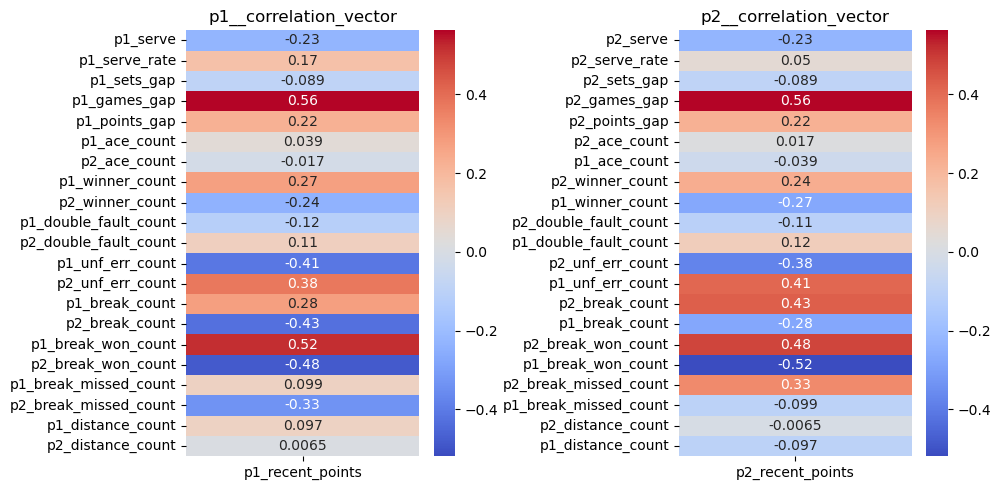
\includegraphics[width=0.85\textwidth]{./graph/final_game_relationship.png}
    \caption{Correlation Analysis between Player performance and Match Parameters (Finals)}
\end{figure}

As the final featured two players with closely matched skills, we investigated the correlation 
between relevant parameters in the final match and Player 1's performance value. The correlation 
matrix revealed significant associations between player performance and various match factors. 
Notably, there is a strong correlation between player performance and whether the player is serving. 
This underscores the validity of our player performance evaluation function, as it appears capable 
of reflecting changes in various relevant factors throughout the match, thereby capturing the 
overall dynamics of the game.
Next, we will elaborate on the match factors that are highly correlated with Player 1's performance:

\begin{itemize}
    \item \textbf{p1\_server:} Whether Player1 is the server in the current game. This is crucial because the 
    server has a higher chance of scoring. However, if\enspace Player1 is the server and does not score in this game, 
    there is a high probability of making a significant mistake, resulting in a noticeable decrease in Player1's 
    performance.
    \item \textbf{p1\_games\_gap:} Difference in the overall score, subtracting opponent's score from Player1's. 
    The correlation coefficient is significant, indicating that the player's performance value will undergo considerable 
    changes when there is a large difference in the overall score. Both players attach great importance to winning 
    or losing this set.
    \item \textbf{p1\_winner\_count, p2\_winner\_count:} Total number of untouchable shots in the last ten games. The 
    correlation coefficients for both are substantial. When Player1 makes a remarkable shot, the audience's mood 
    changes, boosting Player1's morale. Conversely, the opponent's untouchable shots affect Player1's performance.
    \item \textbf{p1\_unf\_err\_count, p2\_unf\_err\_count:} Total number of mistakes in the last ten games. 
    Excessive personal mistakes can affect Player1's mentality and indicate a poor performance. However, opponent 
    mistakes mean more opportunities for Player1, leading to a smoother game and increased points. Player1's performance 
    is enhanced with more points.
    \item \textbf{p1\_break\_count, p2\_break\_count:} Number of break points in the last ten games. The positive 
    correlation suggests that a break indicates a chance for Player1 to win the game. Player1 tends to make 
    more effort and has a better performance. Conversely, the opponent's break points affect Player1's performance, leading to 
    possible nervousness and mistakes.
\end{itemize}

\subsection{\textbf{Application of Player Performance Evaluation Model}}

To further illustrate the validity of our model, we applied the player performance function to a 
specific match. We chose the men's singles final of the 2023 Wimbledon Championship, featuring 
Novak Djokovic against Alcaraz. This match is considered the most evenly matched and 
representative. The graph below shows the fluctuation of the two players' performances:

\begin{figure}[H]
    \centering
    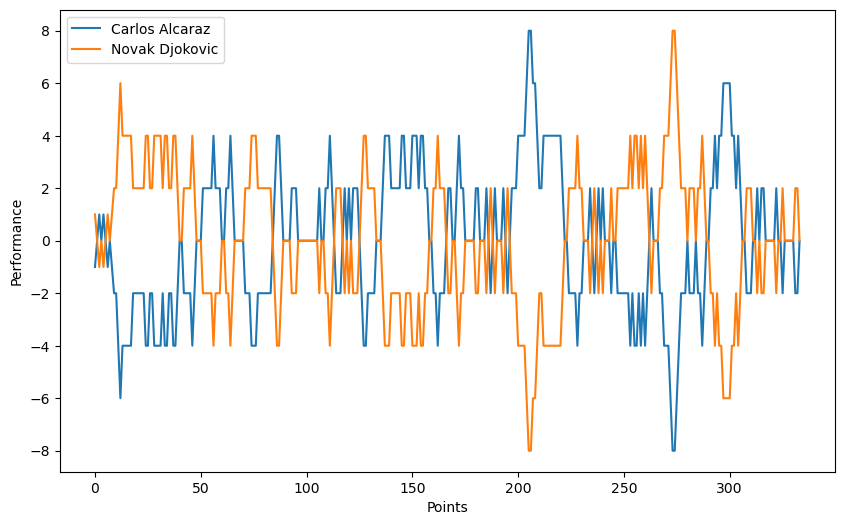
\includegraphics[width=0.75\textwidth]{./graph/performance.png}
    \caption{Application of Player performance Evaluation Function in the Final (All Matches)}
\end{figure}

The match between Djokovic and Alcaraz was a thrilling five-setter. Djokovic started strong, 
taking the first set, but Alcaraz quickly responded by winning the second. The momentum shifted 
noticeably in the third set, with Alcaraz dominating to take a lead. Although Djokovic managed 
to tie the match by winning the fourth set, Alcaraz secured victory in the decisive fifth set 
with a score of 6-4.
Analyzing the player performance curves, we see that Djokovic had a higher performance level 
than Alcaraz at the beginning of the match, particularly in the first set where his performance 
slightly dipped after losing a point but remained high until around the 50-point mark. The 
second set showed a more contested scenario, with the performance curves intersecting 
frequently, highlighting a highly competitive phase that extended into a tiebreak. Alcaraz's 
performance soared in the third set, culminating in a 6-1 victory, which indicated a 
significant momentum shift in his favor.
Djokovic rallied in the fourth set, his performance improving notably around the 273rd point, 
demonstrating his resilience and ability to bounce back. Nevertheless, the fifth set saw 
Alcaraz maintaining a slight edge, with both players' performance curves remaining close until 
Alcaraz ultimately clinched the match.

\section{\textbf{Turning Point Prediction Model}}
\subsection{\textbf{Definition of Match Turning Points}}

Firstly, let's define the turning points of a match. When one player wins a game, wins a set, 
loses the previous point and wins the following three points, we consider it a turning point 
in the match. To clearly identify whether the support shifts from one player to another, we 
introduce a variable $S_t$. When Player 1 wins a game, wins a set, loses the previous point 
and wins the following three points $S_t=1$. Similarly, when Player 2 achieves the same 
conditions $S_t=-1$. In other cases $S_t$ remains unchanged. When $S_t$ changes from 1 to -1, 
the match shifts its support from Player 1 to Player 2. When $S_t$ changes from -1 to 1, 
the match shifts its support from Player 2 to Player 1. When $S_t$ remains unchanged, no 
turning point occurs.

Next, we define the variables and the predicted values used. Using $S_t$ as the predicted 
value, it can determine if the current situation is a turning point. The calculation is as 
follows:

\begin{table}[H]
    \caption{Definition of Turning Point $S_t$}
    \centering
    \begin{tabular}{|c|c|c|c|}
    \hline
    The value of $S_t$ & $S_{t-1}$ & 1 & -1  \\ \hline
    \multirow{5}{*}{Situation} &  & $p1\_games\_t<p1\_games\_t+1$ & $p2\_games\_t<p2\_games\_t+1$ \\ \cline{3-4}
     & If the match data & $p1\_sets\_t<p1\_sets\_t+1$ & $p2\_sets\_t<p2\_sets\_t+1$  \\ \cline{3-3} \cline{3-4} 
     & is not in the right & $points\_victor\_t+1=1$ & $points\_victor\_t+1=2$  \\
     & side situation & $points\_victor\_t+2=1$ & $points\_victor\_t+2=2$  \\
     &  & $points\_victor\_t+3=1$ & $points\_victor\_t+3=2$  \\ \hline
    \end{tabular}
\end{table}

On the other hand, we select the current and previous states of the match as variables to 
predict if the match is about to undergo a turning point. These include: $p1\_scores$, 
$p2\_scores$, $scores\_diff\_count$, $p1\_server$, $p1\_recent\_points$, $p2\_recent\_points$, 
$run\_diff\_count$, $p1\_ace\_count$, $p2\_ace\_count$, $p1\_winner\_count$, $p2\_winner\_count$, 
$p1\_unf\_err\_count$, $p2\_unf\_err\_count$, $p1\_break\_count$, $p2\_break\_count$,\\ 
$p1\_break\_won\_count$, $p2\_break\_won\_count$. The selection of these variables is based on 
our understanding of the match and the evaluation of the player's state. We believe these 
variables can effectively reflect the trend of the match.

\subsection{\textbf{Building the Model for Predicting Turning Points}}
We use the logistic regression model to construct our entire model. Logistic regression is a binary classification 
model used to predict the outcome of an event as one of two possible outcomes. It is based on the principle of 
linear regression, mapping the result of a linear combination to the probability range (between 0 and 1), and then 
classifying based on a set threshold. In this case, we perform linear regression on the variables of the match, 
predicting the value of \(S_t\) through probability transformation and decision threshold. Logistic regression 
learns the weights \(w_i\) by minimizing the loss function.

By conducting logistic regression across all matches, we obtain the weights for each variable, from \(p2\_scores\) to \(p2\_break\_won\_count\), denoted as \(x_i (i=1…17)\), and their weights are shown in the figure below:

\begin{figure}[H]
    \centering
    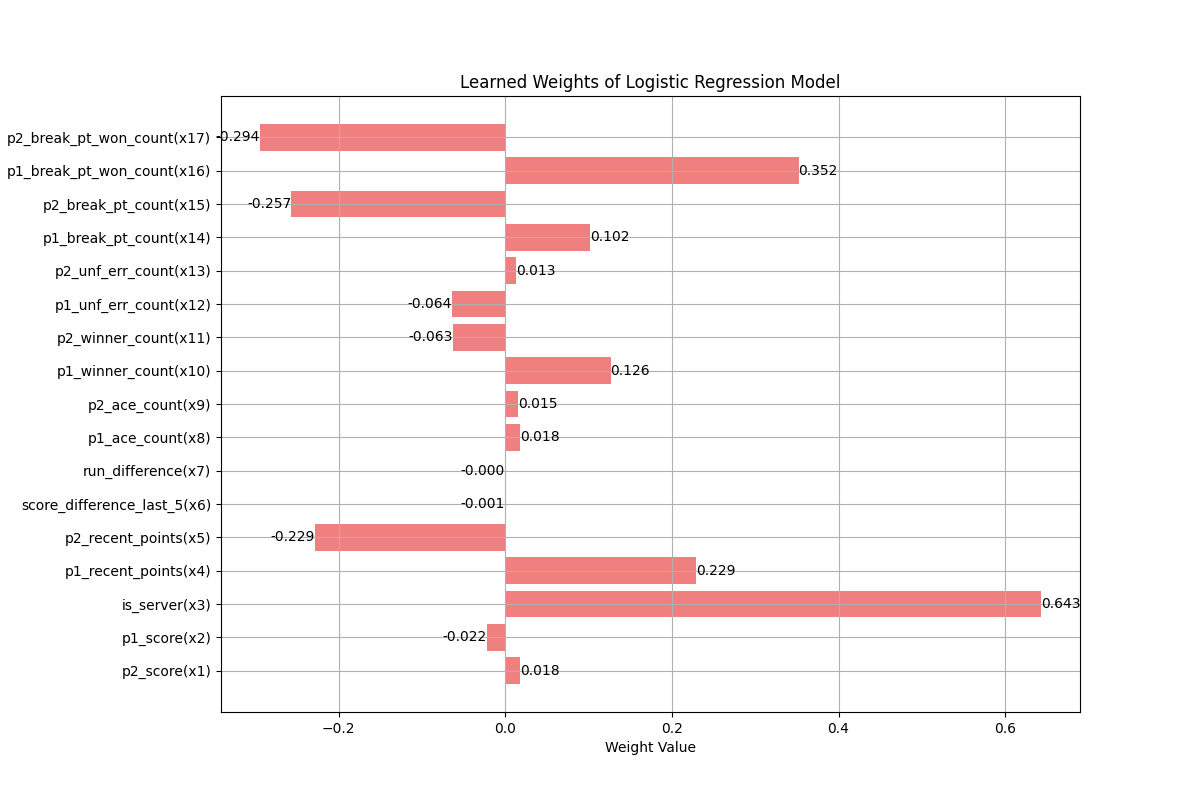
\includegraphics[width=\textwidth]{./graph/weights.png}
    \caption{Weights of Variables in the Logistic Regression Model}
\end{figure}

This leads us to the linear combination function:
\[z = b + \sum_{i=1}^{17}w_ix_i\]
which undergoes a probability transformation:
\[g(z) = \frac{1}{1 + e^{-b - \sum_{i=1}^{17}w_ix_i}}\]
Finally, the prediction of \(S_t\) is made based on the decision threshold:
\[ \text{if}\ g(z) > 0.5, \quad S_{t_{pred}} = 1 \]
\[ \text{if}\ g(z) < 0.5, \quad S_{t_{pred}} = -1 \]
Thus, our prediction formula becomes:
\[S_{t_{pred}} = 2\left(f\left(\frac{1}{1 + e^{-b - \sum_{i=1}^{17}w_ix_i}}\right)\right) - 1\]
The accuracy of the logistic regression model is defined as:
\[Accuracy = \frac{Total\ Number\ of\ Correct\ Predictions}{Total\ Number\ of\ Predictions}\]
In the test set, our model achieved an accuracy of 0.75, indicating that our prediction accuracy for turning 
points reached 75\%, which is a commendable level.

Following this, we conduct a correlation test between turning points and these variables. The Pearson correlation 
coefficient is given by:
\[r = \frac{\sum_{i=1}^{n}(X_i-\overline{X})(Y_i-\overline{Y})}{\sqrt{\sum_{i=1}^{n}(X_i-\overline{X})^2}\sqrt{\sum_{i=1}^{n}(Y_i-\overline{Y})^2}}\]
It measures the strength and direction of the linear relationship between two variables. The value ranges from -1 
to 1: 1 indicates a perfect positive correlation, while -1 indicates a perfect negative correlation. Correlation 
tests can help us determine which variables have a stronger or weaker relationship with the occurrence of turning 
points.

\begin{figure}[H]
    \centering
    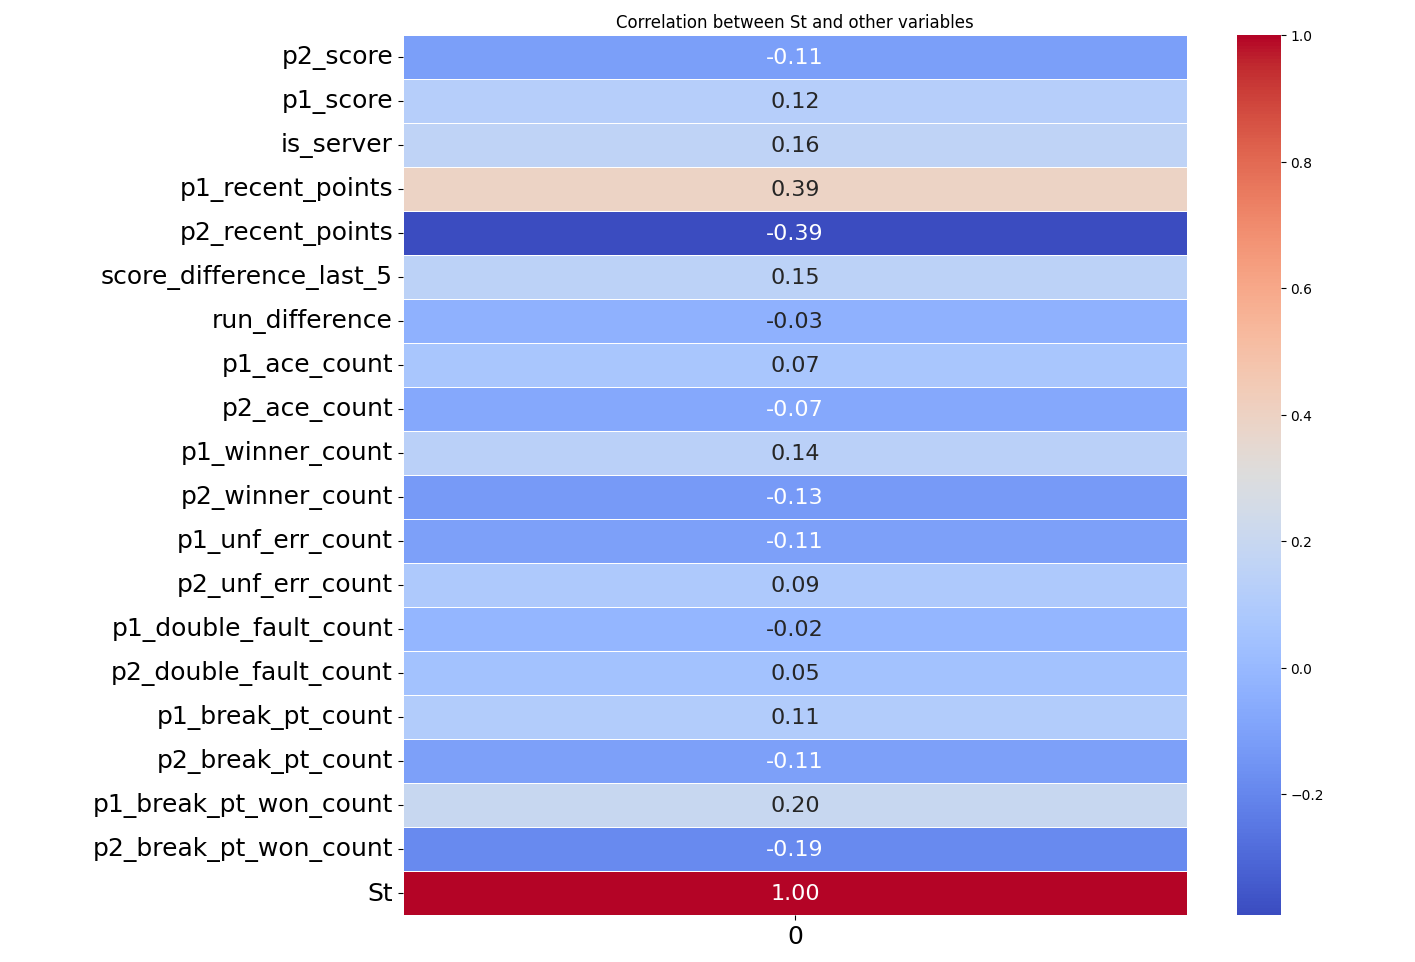
\includegraphics[width=\textwidth]{./graph/relativity.png}
    \caption{Corralation between Variables and $S_t$}
\end{figure}

From the graph, we can identify several variables that have a significant relationship with \(S_t\), specifically 
those with an absolute correlation value greater than 0.15. These variables, in descending order of their 
correlation, are \(p1\_recent\_points\), \(p2\_recent\_points\), \(p1\_server\), \(scores\_diff\_count\), 
\(p1\_break\_won\_count\), \(p2\_break\_won\_count\), \(p1\_winner\_count\), and \(p2\_winner\_count\). 
These include the recent scoring situation of players 1 and 2, the current server, whether players 1 and 2 have 
recently succeeded in breaking serve, and the number of untouchable shots recently made by players 1 and 2. The 
linear combination of these variables can be used to measure a player's current performance and predict the 
occurrence of turning points. Thus, we define a player's momentum as:
\[momentum = b + \sum_{i=1}^{17}w_ix_i\]

\subsection{\textbf{Application of the Turning Point Prediction Model}}
\subsubsection{\textbf{Non-randomness of Turning Points}}
Based on our definition of turning points, we can quantitatively describe the dynamics of a match. We 
choose the match with \(match\_id = 1701\), namely the final between Alcaraz and Djokovic. Below is the 
graph we produced showing the changes in \(S_t\) with the scoring events of this match:

\begin{figure}[H]
    \centering
    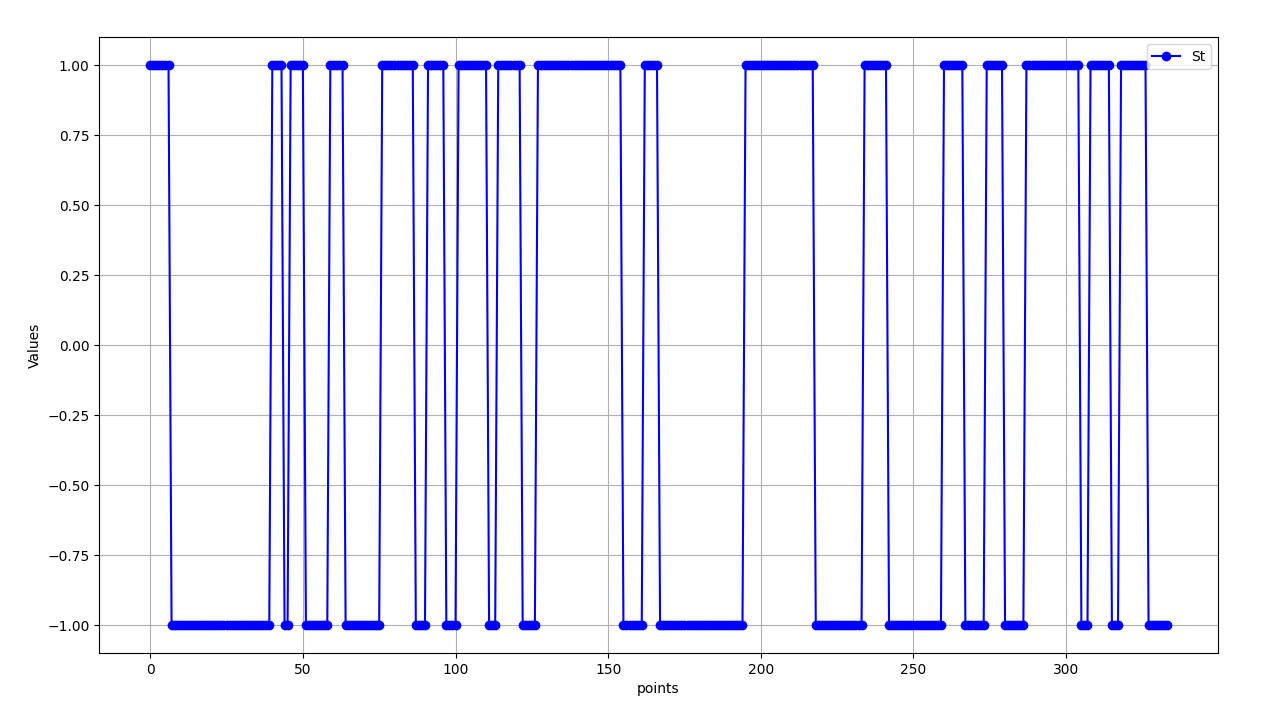
\includegraphics[width=0.95\textwidth]{./graph/true_swings.png}
    \caption{Changes in Turning Points \(S_t\) with Scoring Events in the Final}
\end{figure}

Now, we apply the runs test to analyze the randomness of \(S_t\) values. In this context, a run is 
defined as a sequence of consecutive 1s or -1s. Assuming \(S_t\) is a random sequence, and given a 
sufficiently large number of points, the central limit theorem suggests that the number of runs \(R\) 
follows a normal distribution, with the expected value and standard deviation of \(R\) given by:
\[E(R) = \frac{2 \times N_1 \times N_2}{N} + 1\]
\[\sigma(R) = \sqrt{\frac{2 \times N_1 \times N_2 \times (2 \times N_1 \times N_2 - N)}{N^2 \times (N - 1)}}\]
We calculate the Z-value using the actual observed number of runs and its standard deviation:
\[Z = \frac{observed\ runs - expected\ runs}{\sigma(R)}\]
Applying this Z-value for the test, we obtain a Z-value and a P-value $$Z = -11.09558,\enspace P = 1.31807\times 10^{-28}$$ 
Given that the P-value is significantly less than 
0.05, we reject the null hypothesis, suggesting that the turning points in the match are not random and 
are influenced by certain factors.

Next, we will demonstrate that this factor largely depends on the player's "momentum." We select 
the variables with high correlation identified earlier and use the logistic regression model to 
predict the \(S_t\) values for this match. The results are as follows:

\begin{table}[H]
    \caption{Turning Point Model Prediction Report}
    \centering
    \begin{tabularx}{0.95\textwidth}{XXXXX}
    \toprule
    \multicolumn{5}{c}{Classification Report:}\\
    \midrule
     & Precision & Recall & F1-Score & Support \\
    -1 & 0.69 & 0.64 & 0.67 & 14  \\
    1 & 0.82 & 0.85 & 0.84 & 27  \\ 
    \midrule
    Accuracy &  &  & 0.78 & 41  \\
    Macro Avg & 0.76 & 0.75 & 0.75 & 41  \\
    Weighted Avg & 0.78 & 0.78 & 0.78 & 41  \\
    \bottomrule
    \end{tabularx}
\end{table}

As seen, the model achieves a prediction accuracy of 0.78. Next, we compare the predicted \(S_t\) 
values with the actual \(S_t\) values:

\begin{figure}[H]
    \centering
    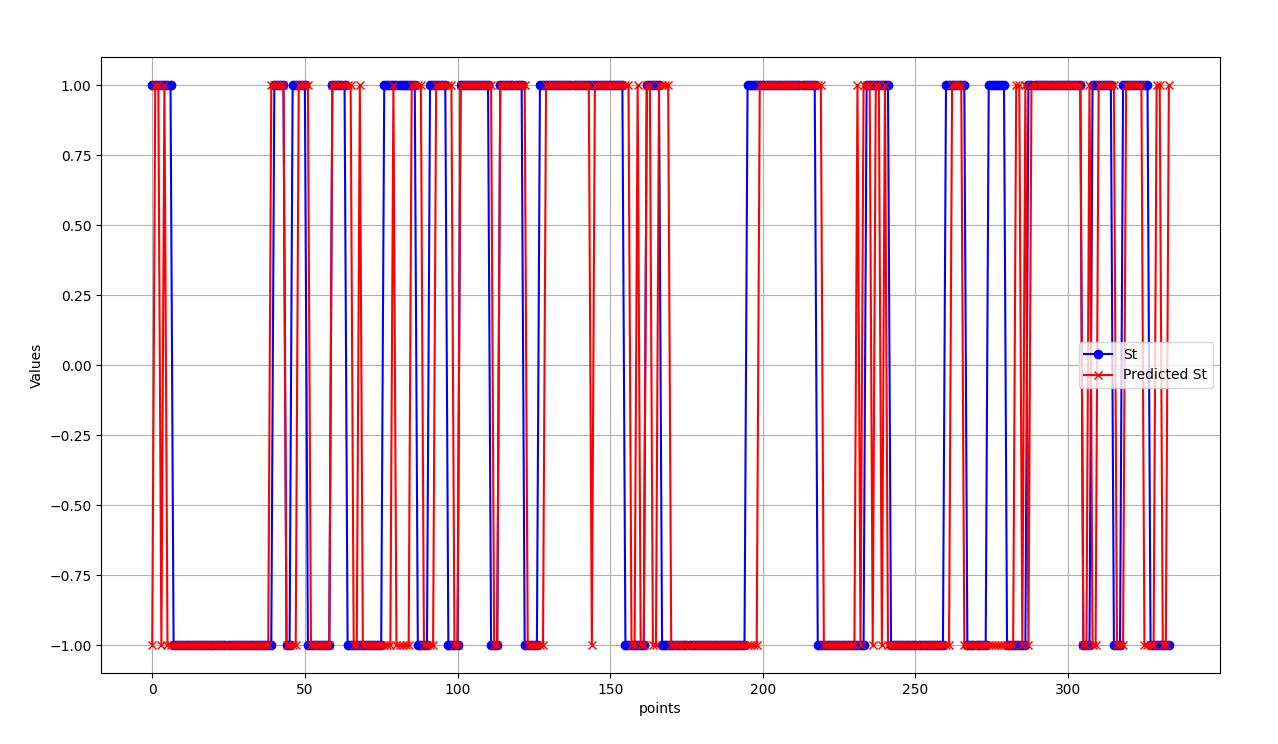
\includegraphics[width=\textwidth]{./graph/predict_swings.png}
    \caption{Comparison of Predicted and Actual Turning Points \(S_t\) in the Final Match}
\end{figure}

From the curve, we can observe that although there are some fluctuations in the predicted values, the 
overall trend aligns closely with the actual values, especially during the phases around the 50th and 
100th points where both players performed noticeably well. Next, we calculate the correlation coefficient 
between the set of predicted \(S_t\) values and the actual values to further elucidate their relationship. 
We computed the Pearson Correlation with the results as follows:

\begin{table}[H]
    \caption{Calculated Results for Correlation Coefficients}
    \centering
    \begin{tabular}{|c|c|}
    \hline
     & Pearson Correlation \\ \hline
    Correlation & $0.52196$ \\ \hline
    P\_value & $1.92580\times10^{-15}$ \\ \hline
    \end{tabular}
\end{table}

Additionally, we calculated the Jaccard similarity between the two sets, which measures their similarity 
by the ratio of the number of elements in their intersection to the number of elements in their union. 
The calculation formula is as follows:
\[J(A,B) = \frac{|A \cap B|}{|A \cup B|}\]
The calculation resulted in \(0.625\), indicating a high degree of similarity between the two sets. These 
correlation calculations all suggest a strong correlation, thus indicating that the turning points in a 
match are not random and are significantly correlated with the "momentum" we defined earlier.

\subsubsection{\textbf{Assistance in Match Preparation}}
Considering that the momentum of different players is affected by various factors differently, we aim to 
identify the factors that have the most significant impact on a specific player to provide preparation 
suggestions. Therefore, we can use the match data of a specific player to train, derive their specific 
momentum function, and analyze the parameters. Here, we analyze two matches of the champion Carlos Alcaraz.

\begin{figure}[H]
    \centering
    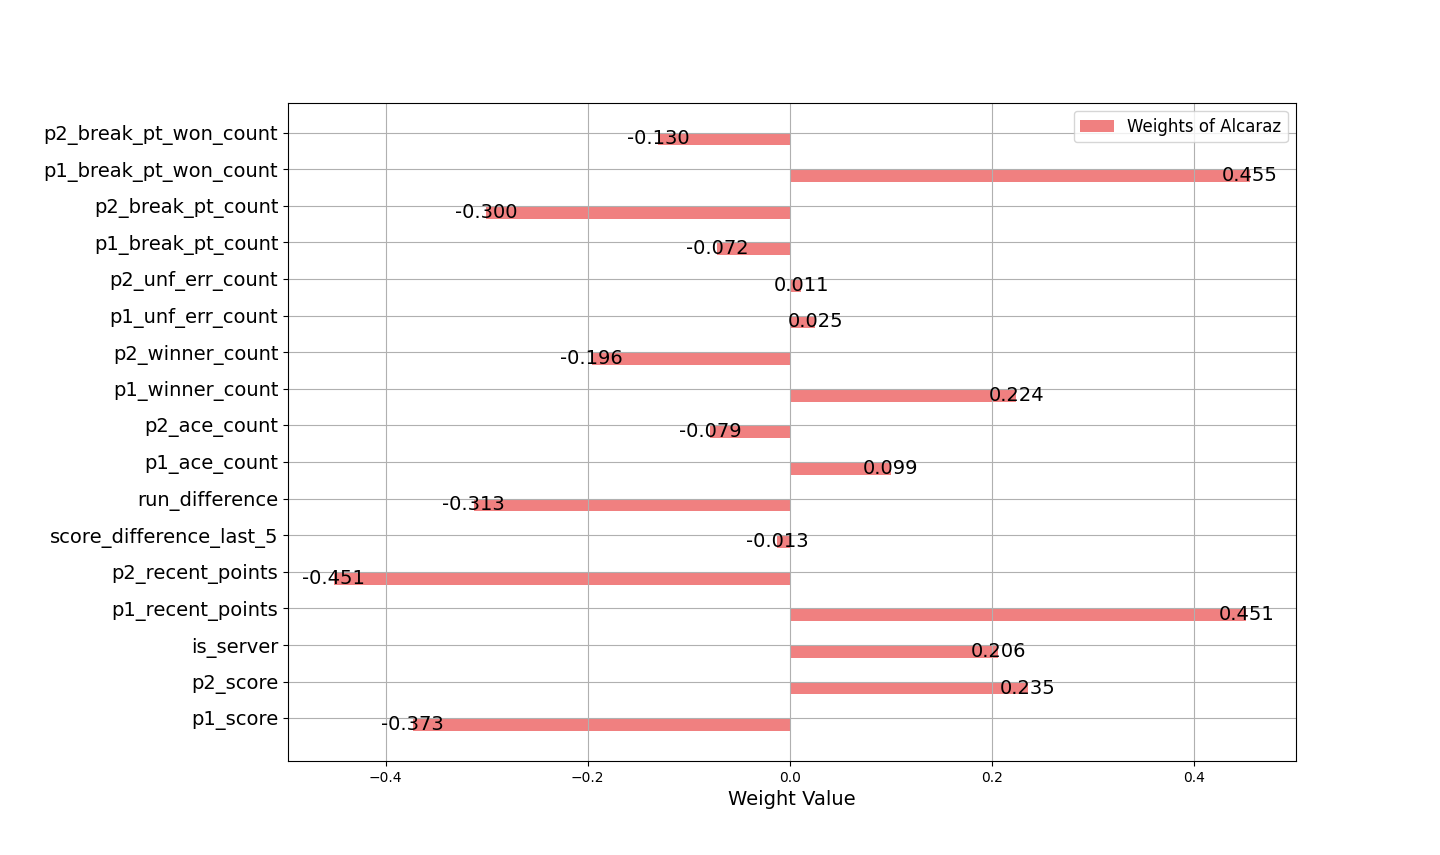
\includegraphics[width=0.95\textwidth]{./graph/champion.png}
    \caption{Variable Weights in Matches for Alcaraz}
\end{figure}
From the figure, we can see that Alcaraz's match momentum is mainly influenced by \(p1\_recent\_points\) 
and \(p2\_recent\_points\), that is, the recent scoring performance of him and his opponent. Additionally,\\ 
\(break\_pt\_won\_count\) significantly boosts his match momentum. Whether serving, scoring on serve, and 
making impressive shots also significantly impact his match state. Notably, errors have a minor impact on 
a player's momentum, indicating strong mental resilience, which is a key reason for his victory over 
Djokovic.

To highlight the differences in momentum-impacting factors between players, we also trained and analyzed 
another player, Novak Djokovic. Comparing the factors affecting the momentum of the two players, we observed:

\begin{figure}[H]
    \centering
    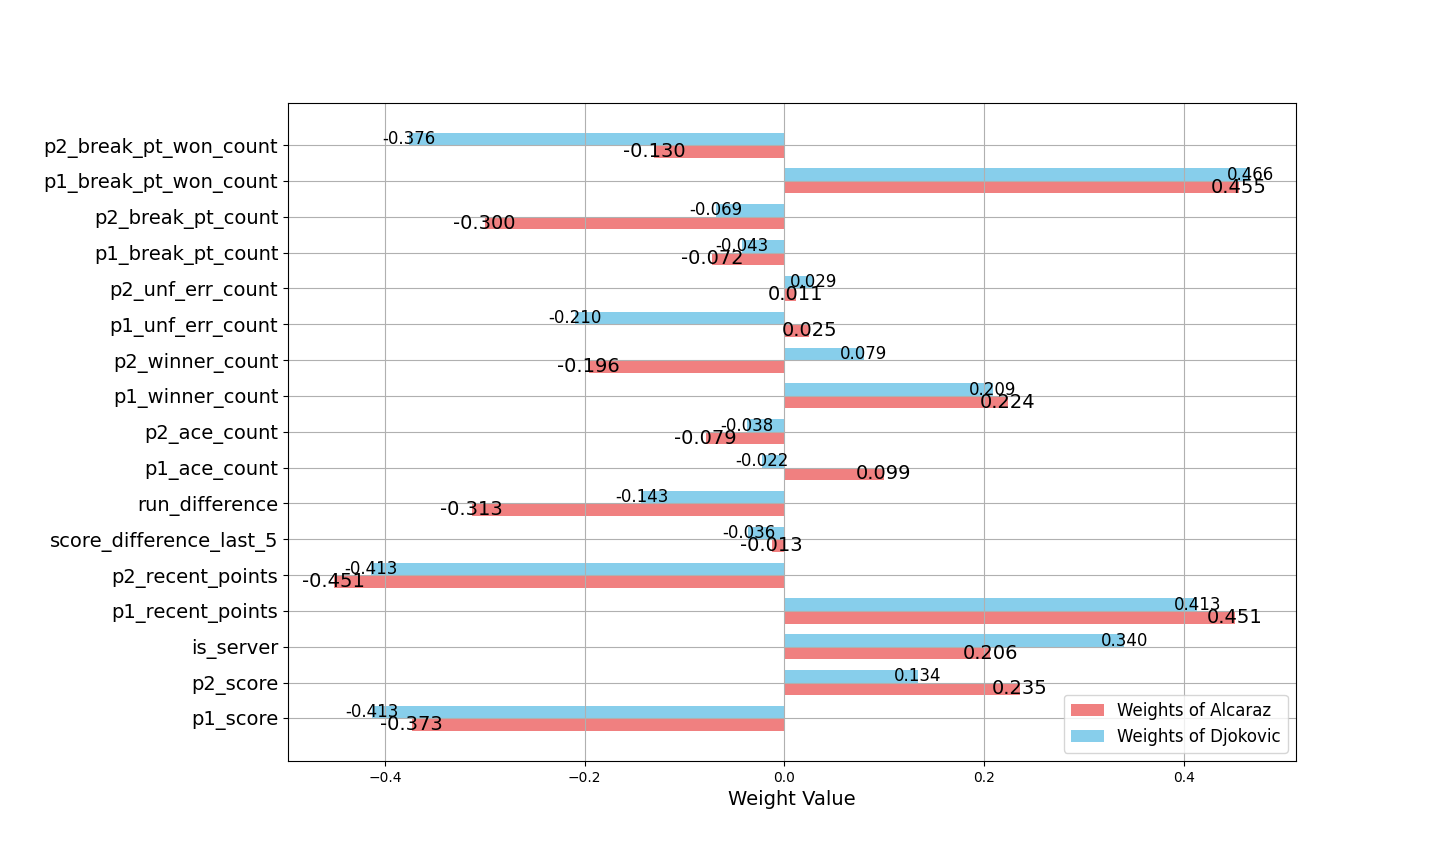
\includegraphics[width=\textwidth]{./graph/final_game.png}
    \caption{Comparison of Variable Weights in the Final Match between Alcaraz and Novak Djokovic}
\end{figure}

It is observed that most indicators have similar weights for both players, but whether serving and scoring 
on serve have a greater impact on Novak Djokovic. Moreover, Novak Djokovic is more affected by his own 
errors and the opponent gaining break points, which could be a significant reason for his loss in the 
third set to Alcaraz by 1-6.

Combining these factors, we can offer some suggestions to players. First, it is essential for a player to 
understand which factors are most closely related to their momentum. For instance, for Djokovic, avoiding 
unforced errors and the opponent's break points might be crucial for maintaining a positive mindset, as 
well as leveraging his serving advantage.

Secondly, players need to comprehend the momentum characteristics of their opponents. For example, when 
facing Alcaraz, one should be wary of him scoring consecutive points leading to significant comebacks. 
Considering the impact of running distance on Alcaraz's momentum, adopting a strategy to wear him down 
with long shots could be beneficial. In summary, we can provide tailored advice based on the different 
momentum-impacting factors of each player.

%----------------------------------------------------------------------------------


% 稳定性分析
%----------------------------------------------------------------------------------
\section{\textbf{Stability Analysis}}
Using different training data, such as four matches of Carlos Alcaraz, four of Novak Djokovic, three 
of Andrey Rublev, three of Jannik Sinner, and three of Roman Safiullin, we calculated the model's 
accuracy. We also compared several important factors like \(is\_server\), \(p1\_score\), 
\(p1\_recent\_points\), \(p1\_ace\_count\), \(p1\_winner\_count\), and \(p1\_break\_won\_count\) 
(since \(p1\) and \(p2\) parameters are symmetrical, we only use \(p1\) parameters here) against the 
model parameters obtained from training on all data. Different players' detailed parameters are listed in the appendices. The results are as follows:

\begin{table}[H]
    \caption{Model Training Results on Different Datasets}
    \centering
    \begin{tabular}{|c|c|c|c|c|c|c|}
    \hline
     & Carlos & Novak & Andrey & Jannik & Roman & All \\
     & Alcaraz & Djokovic & Rublev & Sinner & Safiullin & Games \\ \hline 
    Model Accuracy & 0.72 & 0.73 & 0.74 & 0.69 & 0.79 & 0.67 \\ \hline
    Parameter (\(is\_server\)) & 0.206 & 0.340 & 0.203 & 0.216 & 0.175 & 0.239 \\ \hline
    \(p1\_score\) & -0.373 & -0.413 & 0.222 & 0.207 & -0.556 & 0.200 \\ \hline
    \(p1\_recent\_points\) & 0.451 & 0.413 & 0.445 & 0.331 & 0.482 & 0.229 \\ \hline
    \(p1\_ace\_count\) & 0.099 & -0.022 & 0.077 & 0.249 & 0.376 & 0.070 \\ \hline
    \(p1\_winner\_count\) & 0.224 & 0.209 & 0.110 & 0.290 & 0.231 & 0.140 \\ \hline
    \(p1\_break\_won\_count\) & 0.455 & 0.466 & 0.655 & 0.582 & 0.492 & 0.544 \\ \hline
    \end{tabular}
\end{table}

We observed that the Model Accuracy obtained from different datasets is quite close, all around 0.7. 
The parameters \(is\_server\), \(p1\_recent\_points\), and \(p1\_break\_won\_count\) show high 
stability (as highlighted in the table), with overall deviations from the all-data trained parameters 
of 0.012, 0.195, and 0.010, respectively. This indicates that these parameters have a similar impact 
on each player, suggesting their universal influence on match momentum.

% Model Evaluation and Further Discussion
\section{\textbf{Model Evaluation and Further Discussion}}
\subsection{\textbf{Strengths and Weaknesses}}

\noindent\textbf{Strengths:}
\begin{itemize}
    \item High model accuracy, with the defined momentum showing significant correlation with various 
    match data, and the accuracy of the actual match prediction is greater than 0.6.
    \item The momentum formula obtained from the model can be scientifically explained, such as the 
    advantage of serving, and the impact of scoring and errors on a player's mentality.
    \item The model can analyze the factors affecting different players' momentum individually, 
    helping them to understand themselves and their opponents.
\end{itemize}

\noindent\textbf{Weaknesses:}
\begin{itemize}
    \item Limited training data, using only over seven thousand points provided in the dataset, which 
    does not test the model's performance with more data.
    \item The defined momentum lacks significant correlation with some match variables such as player 
    errors, running distance, serve direction, and return depth, possibly due to insufficient 
    consideration of factors.
    \item The model does not consider variables like set and match scores, which significantly impact 
    a player's mentality and pressure.
\end{itemize}

\subsection{\textbf{Further Discussion}}
We applied the previously derived turning point prediction formula
\[S_{t_{pred}} = 2\left(f\left(\frac{1}{1 + e^{-b - \sum_{i=1}^{17}w_ix_i}}\right)\right) - 1\]
to five matches from the 2023 Wimbledon, repeating the above work to predict the turning point changes 
throughout the matches based on relevant data and comparing them with the actual turning points using 
the Jaccard similarity test. The model's Jaccard accuracy rates are as follows:

\begin{table}[H]
    \caption{Model Jaccard Accuracy for Other Matches}
    \centering
    \begin{tabular}{|c|c|c|c|c|c|}
    \hline
    Match & 1301 & 1401 & 1501 & 1601 & 1701 \\ \hline
    Accuracy & 0.674 & 0.650 & 0.663 & 0.677 & 0.607 \\ \hline
    \end{tabular}
\end{table}

The model's Jaccard accuracy rate is approximately between 0.6-0.7, with minor fluctuations in prediction 
accuracy for different matches, notably a slightly lower accuracy for the final match. When applied to 
other matches, the overall accuracy is relatively high, and the predictions somewhat align with the actual 
outcomes. However, the dataset used for model training is not very large, leading to some randomness: the 
frequency of matches between any two players is limited, and data can vary significantly between players. 
Higher-level players may have a lower probability of making mistakes, which could reduce the impact of 
certain variables. These factors diminish the model's universality, suggesting that when applying it to 
matches between different players, the choice of parameters may need adaptation. Ideally, a specific model 
should be constructed for a specific player, analyzing past match data to determine which parameters 
should be used as independent variables for training the model.

When applying the model to other types of matches or sports, it is necessary to select data based on the 
characteristics of each game, requiring manual data preprocessing and reprocessing. The specific process is as follows:

\begin{figure}[H]
    \centering
    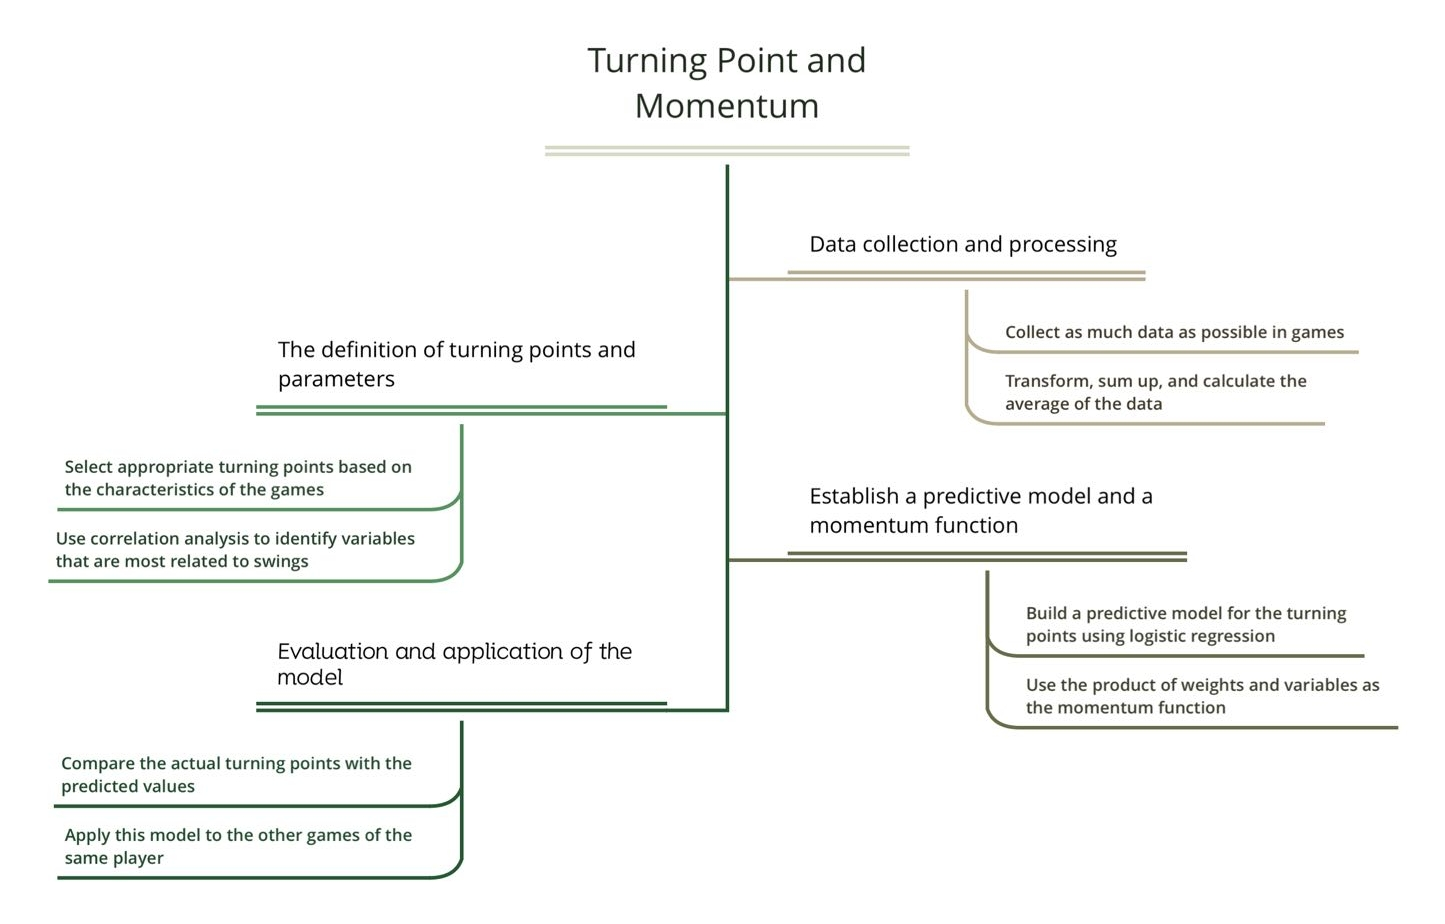
\includegraphics[width=0.95\textwidth]{./graph/flow_chart.jpg}
    \caption{Process for Establishing a Turning Point Model for Any Match}
\end{figure}

Identifying turning points and selecting parameters are crucial, as data processing will vary based on the 
distinctive features of each sport. For example, in volleyball matches, the serving side does not have an 
inherent advantage, contrary to what might be expected, due to the strategic setups by the opposing team. 
The number of passes, spikes, and the height of blocks are important parameters in volleyball, unlike in 
tennis. Even within the same sport, different levels of competition may focus on different aspects, and 
players' tactics may vary. These are all considerations. Once turning points and parameters are determined, 
building the model and obtaining a momentum function becomes straightforward.

%----------------------------------------------------------------------------------


% Conclusion 总结
%----------------------------------------------------------------------------------
\section{Conclusion}
This article presents a formula reflecting recent player performance, analyzing its correlation with various match factors, and identifying variables with strong correlations. 
Utilizing these strongly correlated factors as variables and treating match turning points as prediction values, a logistic regression model was employed for training, 
achieving high accuracy on the test set. Consequently, formulas for assessing player momentum and predicting turning points were obtained. 
A correlation matrix was constructed to depict the relationships between turning points and these match factors, identifying the most predictive elements.

The derived turning point prediction formulas were applied to multiple matches, revealing a high similarity with actual values. This suggests that the turning point prediction formulas exhibit high accuracy in the majority of matches, 
effectively forecasting turning point occurrences. The study subjected actual turning points in a match to a run test, comparing them with predicted turning points, 
and discovering non-random occurrences. Furthermore, logistic regression was applied to predict specific player performances, 
analyzing individual strengths and weaknesses to formulate corresponding strategies.

However, in some matches, the precision of the turning point prediction formulas appears less accurate, potentially due to the oversight of certain match factors. 
Factors such as the current game and set scores, variations in player skill levels, match duration, serve success rate, and return quality were not considered. 
Additionally, the model's performance varied based on the selection of different match parameters and the definition of turning points, 
emphasizing the need to refine variable selection for enhanced universality.

%----------------------------------------------------------------------------------


% Memo to the coaches 给教练的备忘录
%----------------------------------------------------------------------------------
\section{Memo}

\noindent Memo \\
TO: Coaches of Tennis games \\
FROM: Team \# 2416996 \\
DATE: February 5, 2023 \\
SUBJECT: Research on 'Momentum' in Tennis Games \\
\hrule
\vspace{0.5cm}
\noindent Dear Coach,

We modeled the "momentum" of players during the 2024 Wimbledon Championships and observed its impact on the course of 
matches. Here are the results of our study and recommendations for athletes:
We analyzed various data points, including the number of points scored, serves made, errors committed, running distance, 
and other factors for each player at specific time points during every match in the 2024 Wimbledon tournament. We examined 
the relationship between these factors and whether the player performed better in the subsequent period. Our findings 
indicated significant correlations between factors such as serving, recent scoring patterns, and the number of impactful 
shots played, with the player's ability to achieve consecutive victories or win matches in the future. This suggests that
 the course of a match is not purely random. Subsequently, we used these factors to construct a model for the players' 
 "momentum." Our model demonstrated high accuracy in predicting match outcomes, exceeding 70\%.
Furthermore, we identified that the impact of different factors on the "momentum" varied slightly among different players. 
We provided specific "momentum" models and accuracy assessments tailored to individual players.

In our research paper, we demonstrated that the future course of a match is to some extent influenced by the current 
"momentum" of the players. We identified several key factors affecting this "momentum" and suggested that by analyzing 
these factors, one can predict the direction of a match in advance, providing timely guidance and advice to players.

We conducted a comparative analysis of the differences in the factors influencing the "momentum" of different players. 
We recommend that players, before a match, analyze which factors are most relevant to their own "momentum" during the game 
against their opponents. This analysis helps players understand their strengths and weaknesses. For instance, if a player's "momentum" is significantly influenced by their own mistakes, we advise working on improving psychological resilience when facing errors. Similarly, if a player's momentum is greatly affected by the current server, they should capitalize on their own serving opportunities.
Furthermore, we suggest players analyze the factors influencing the "momentum" of their opponents. If the opponent's 
"momentum" is significantly influenced by serving, one should be cautious of their opponent's serves and take advantage 
of their own serving opportunities. If a decisive shot can boost the opponent's momentum, it is important to focus on 
defense to prevent the opponent from easily making successful shots.

\begin{flushright}
    Yours sincerely,\\
    MCM Team \# 2416996
\end{flushright}
%----------------------------------------------------------------------------------


% References 参考文献
%----------------------------------------------------------------------------------
\addcontentsline{toc}{section}{References} 
\begin{thebibliography}{99} % List your references here
    \bibitem{ref1} Ben Moss \& Peter O'Donoghue (2015) \textit{Momentum in US Open men's singles tennis}. International Journal of Performance Analysis in Sport, 15:3, 884-896, DOI: 10.1080/24748668.2015.11868838
    \bibitem{ref2} Goyal, A., \& Simonoff, J. S. (2020). \textit{Hot Racquet or Not? An Exploration of Momentum in Grand Slam Tennis Matches}. \url{https://arxiv.org/}, 2020.  
    \bibitem{ref3} Dietl, Helmut \& Nesseler, Cornel. (2017). \textit{Momentum in tennis: Controlling the match}. International Journal of Sport Psychology. 48. 10.7352/IJSP2017.48.459. 
    \bibitem{ref4} Richardson, P. A., Adler, W., \& Hankes, D. (1988). \textit{Game, Set, Match: Psychological Momentum in Tennis}. Sport Psychologist, 2(1), 69-76.
    \bibitem{ref5} Henze, Norbert, \& Mathew D. Penrose. (1999). \textit{On the multivariate runs test}. Annals of statistics, 290-298.
    \bibitem{ref6} Gong, Wei, et al. (2014). \textit{On finding the point where there is no return: Turning point mining on game data}. Proceedings of the 2014 SIAM International Conference on Data Mining. Society for Industrial and Applied Mathematics.
    \bibitem{ref7} Menard, Scott. (2002). \textit{Applied logistic regression analysis}. No. 106. Sage.
\end{thebibliography}
%----------------------------------------------------------------------------------


% Appendices 附录
%----------------------------------------------------------------------------------
% List the programming source files of your model and remember to name each file properly.
\newpage
\vspace*{-12ex}
\section*{Appendices}
\addcontentsline{toc}{section}{Appendices} 
\subsection*{Different players' detailed parameters}

\begin{figure}[H]
    \centering
    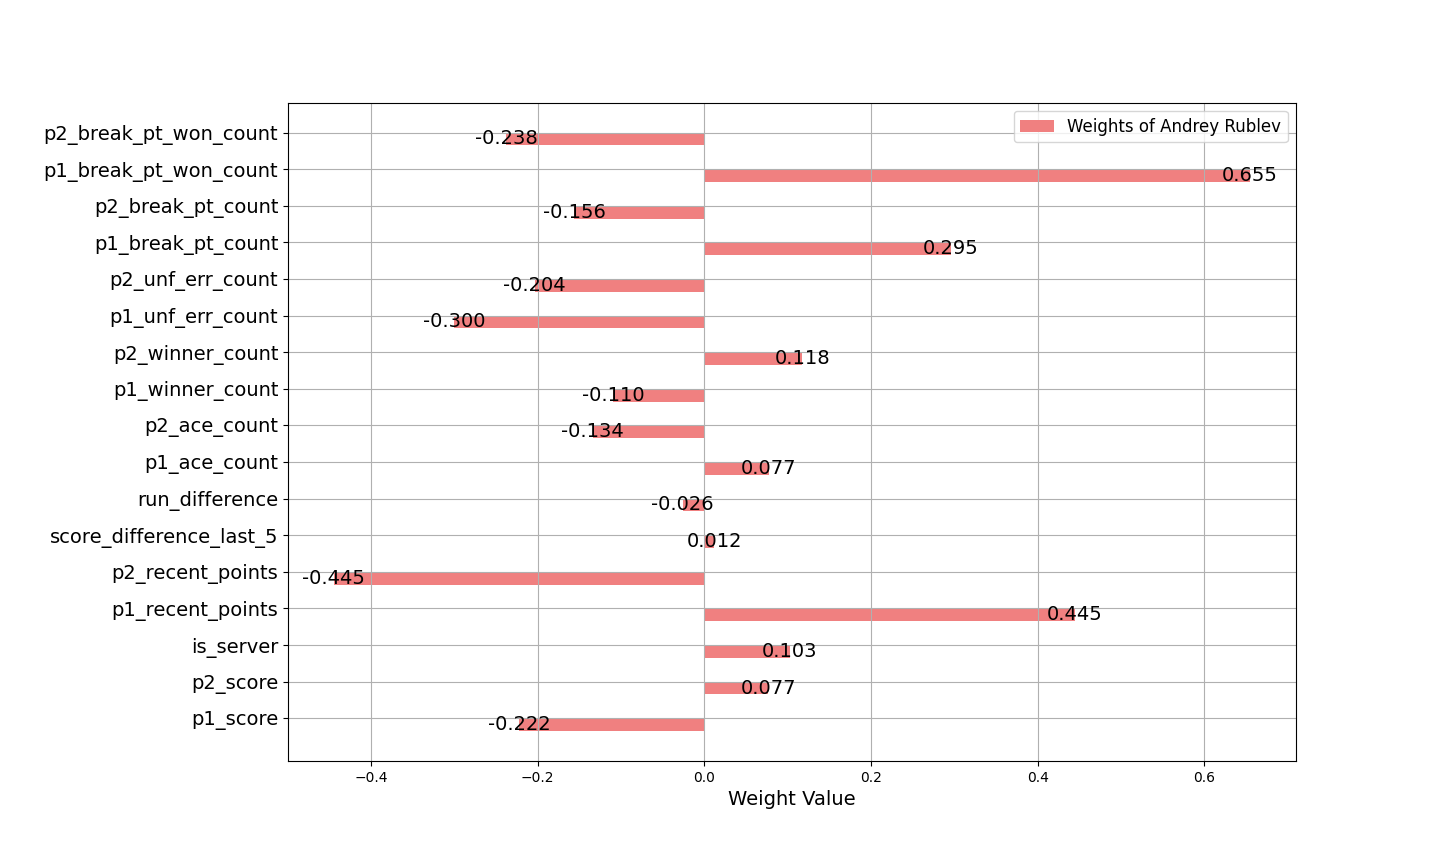
\includegraphics[width=0.6\textwidth]{./graph/Andrey.png}
    \caption{Weights of Andrey Rublev}
\end{figure}

\begin{figure}[H]
    \centering
    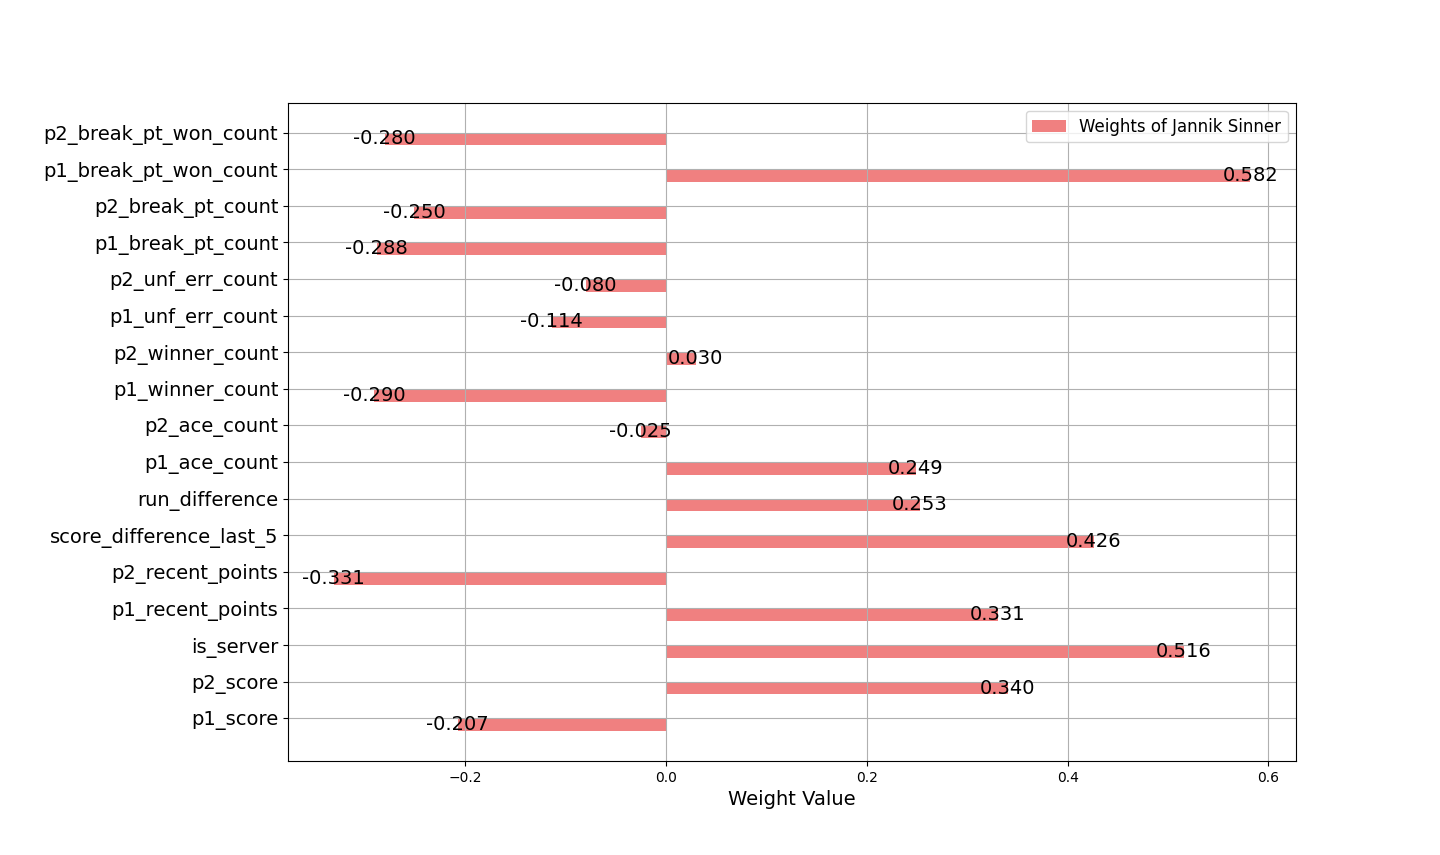
\includegraphics[width=0.6\textwidth]{./graph/Jannik.png}
    \caption{Weights of Jannik Sinner}
\end{figure}

\begin{figure}[H]
    \centering
    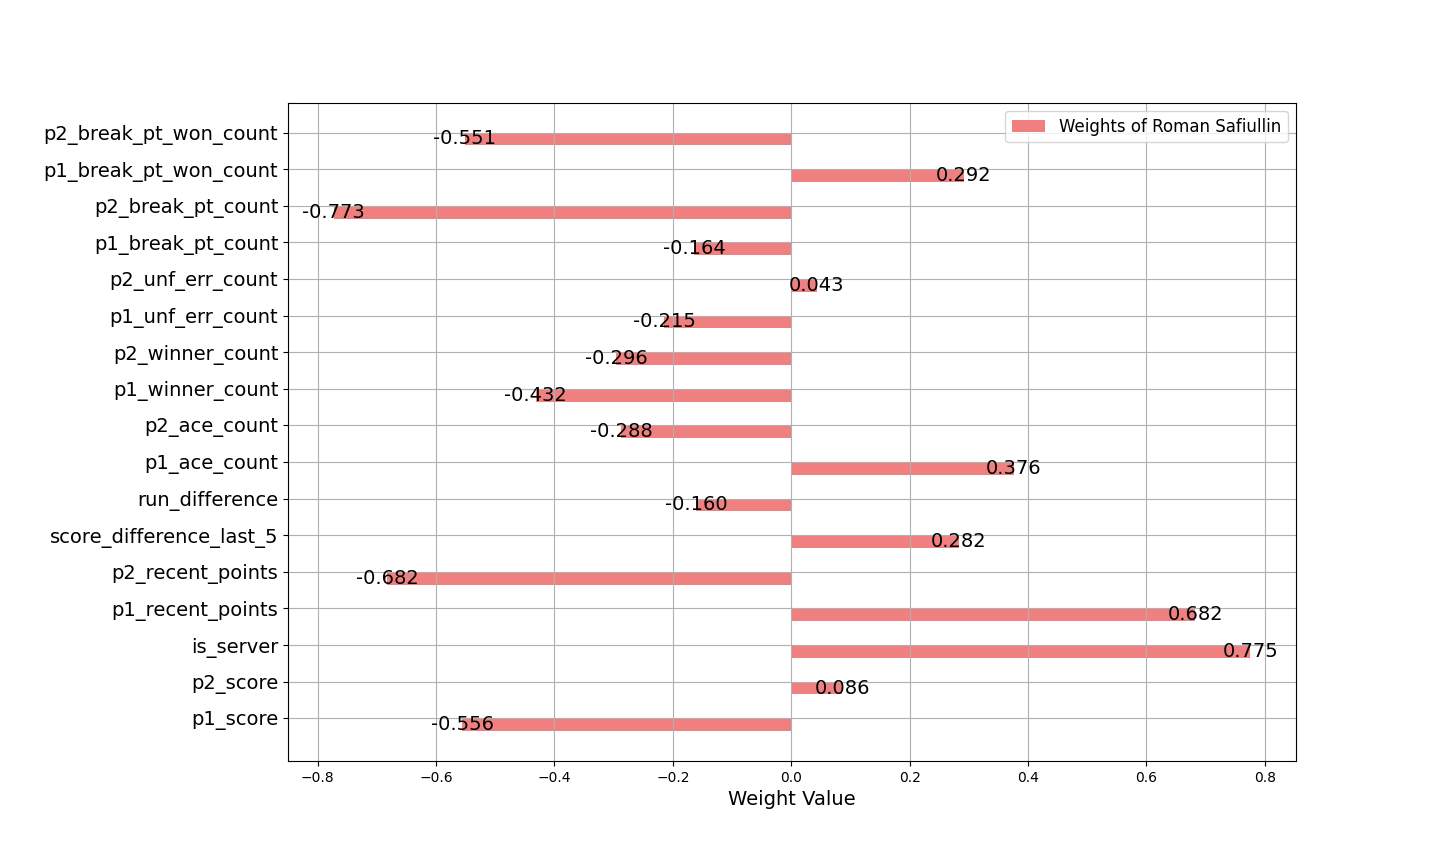
\includegraphics[width=0.6\textwidth]{./graph/Roman.png}
    \caption{Weights of Roman Safiullin}
\end{figure}

\subsection*{Code}
\begin{lstlisting}[language=Python, caption=Code of Data Cleaning and Logistic Regression Model]
    import pandas as pd
    from sklearn.model_selection import train_test_split
    from sklearn.impute import SimpleImputer
    from sklearn.preprocessing import StandardScaler
    # Load the example data
    file_path = r'file_path'
    Data = pd.read_csv(file_path)
    data = Data[Data['match_id'] == '2023-wimbledon-1701']
    # Replace 'AD' with '55' and convert scores to numeric
    data['p1_score'] = data['p1_score'].replace('AD', '55')
    data['p1_score'] = pd.to_numeric(data['p1_score'], errors='coerce')
    data['p2_score'] = data['p2_score'].replace('AD', '55')
    data['p2_score'] = pd.to_numeric(data['p2_score'], errors='coerce')
    # Create a column 'is_point_victor' indicating the player who won the point
    data['is_point_victor'] = 2 - data['point_victor']
    # Add a new column 'recent_points' to record the recent points scored by player 1 and player 2
    data['p1_recent_points'] = (data['point_victor'] == 1).rolling(window=5, min_periods=0).sum() - (data['point_victor'] == 2).rolling(window=5, min_periods=0).sum()
    data['p2_recent_points'] = (data['point_victor'] == 2).rolling(window=5, min_periods=0).sum() - (data['point_victor'] == 1).rolling(window=5, min_periods=0).sum()
    # Quantify non-numeric data
    data['serve_width'] = data['serve_width'].map({'W': 5, 'B/W': 5, 'B': 3, 'B/C': 2, 'C': 1})
    data['serve_depth'] = data['serve_depth'].map({'CTL': 2, 'NCTL': 1})
    data['return_depth'] = data['return_depth'].map({'D': 2, 'ND': 1})
    # Calculate the score difference
    data['score_difference'] = data['p1_score'].astype(str).str.replace('AD', '50').astype(int) - data['p2_score'].astype(str).str.replace('AD', '50').astype(int)
    # Calculate cumulative distance run and run difference
    data['p1_total_distance_run'] = data['p1_distance_run'].cumsum()
    data['p2_total_distance_run'] = data['p2_distance_run'].cumsum()
    data['run_difference'] = data['p1_total_distance_run'] - data['p2_total_distance_run']
    # Create a column 'is_server' indicating the serving player
    data['is_server'] = 2 - data['server']
    # Calculate various rolling statistics
    data['p1_serve_count_last_5'] = (data['server'] == 1).astype(int).rolling(window=5, min_periods=1).sum()
    data['score_difference_last_5'] = data['score_difference'].rolling(window=5, min_periods=1).sum()
    data['p1_ace_count'] = data['p1_ace'].rolling(window=10, min_periods=1).sum()
    data['p2_ace_count'] = data['p2_ace'].rolling(window=10, min_periods=1).sum()
    data['p1_winner_count'] = data['p1_winner'].rolling(window=10, min_periods=1).sum()
    data['p2_winner_count'] = data['p2_winner'].rolling(window=10, min_periods=1).sum()
    data['p1_unf_err_count'] = data['p1_unf_err'].rolling(window=10, min_periods=1).sum()
    data['p2_unf_err_count'] = data['p2_unf_err'].rolling(window=10, min_periods=1).sum()
    data['p1_break_pt_count'] = data['p1_break_pt'].rolling(window=10, min_periods=1).sum()
    data['p2_break_pt_count'] = data['p2_break_pt'].rolling(window=10, min_periods=1).sum()
    data['p1_break_pt_won_count'] = data['p1_break_pt_won'].rolling(window=10, min_periods=1).sum()
    data['p2_break_pt_won_count'] = data['p2_break_pt_won'].rolling(window=10, min_periods=1).sum()
    # Describe turning points in the data
    data['predict'] = 6 - data['point_victor'].shift(-1).fillna(1.5) - data['point_victor'].shift(-2).fillna(1.5) - data['point_victor'].shift(-3).fillna(1.5)
    current_swing = 0
    data['true swings'] = 0
    for index in range(len(data) - 1):
        if index == 0:
            if data['predict'].iloc[index] <= 1:
                current_swing = -1
            elif data['predict'].iloc[index] >= 2:
                current_swing = 1
        else:
            if data['p1_games'].iloc[index] < data['p1_games'].iloc[index + 1]:
                current_swing = 1
            elif data['p2_games'].iloc[index] < data['p2_games'].iloc[index + 1]:
                current_swing = -1
            elif data['p1_sets'].iloc[index] < data['p1_sets'].iloc[index + 1]:
                current_swing = 1
            elif data['p2_sets'].iloc[index] < data['p2_sets'].iloc[index + 1]:
                current_swing = -1
            elif (
                data['p1_points_won'].iloc[index - 1] == data['p1_points_won'].iloc[index]
                and data['p1_points_won'].iloc[index] < data['p1_points_won'].iloc[index + 1]
                and data['p1_points_won'].iloc[index + 1] < data['p1_points_won'].iloc[index + 2]
                and data['p1_points_won'].iloc[index + 2] < data['p1_points_won'].iloc[index + 3]
            ):
                current_swing = 1
            elif (
                data['p2_points_won'].iloc[index - 1] == data['p2_points_won'].iloc[index]
                and data['p2_points_won'].iloc[index] < data['p2_points_won'].iloc[index + 1]
                and data['p2_points_won'].iloc[index + 1] < data['p2_points_won'].iloc[index + 2]
                and data['p2_points_won'].iloc[index + 2] < data['p2_points_won'].iloc[index + 3]
            ):
                current_swing = -1
        data.at[index, 'true swings'] = current_swing
    data.at[index + 1, 'true swings'] = current_swing
    df = pd.DataFrame(data)
    # Split the data into training and testing sets
    X = df[['p2_score', 'p1_score', 'is_server', 'p1_recent_points', 'p2_recent_points', 'score_difference_last_5', 'run_difference', 'p1_ace_count', 'p2_ace_count', 'p1_winner_count', 'p2_winner_count', 'p1_unf_err_count', 'p2_unf_err_count', 'p1_break_pt_count', 'p2_break_pt_count', 'p1_break_pt_won_count', 'p2_break_pt_won_count']]
    # Use SimpleImputer to handle missing values
    imputer = SimpleImputer(strategy='mean')
    X_imputed = imputer.fit_transform(X)  # Remove the last row, as the last row of 'next_point_victor' is NaN
    # Standardize features
    scaler = StandardScaler()
    X_scaled = scaler.fit_transform(X_imputed)
    X_train, X_test, y_train, y_test = train_test_split(X_scaled[:], data['true swings'], test_size=0.2, random_performance=42)
\end{lstlisting} 

\section*{Report On Use of AI}  
\addcontentsline{toc}{section}{Report On Use of AI} 
\subsection*{OpenAI (Nov 5, 2023 version, ChatGPT-3.5,)}
\textbf{Question1:} 
Estimate a logistic regression model for a set of data X and observed outcomes y through Python.

\textbf{Output1:}
from sklearn.model\_selection import\ train\_test\_split\\
from sklearn.linear\_model import LogisticRegression\\
from sklearn.preprocessing import StandardScaler\\
\# Assume X is your feature data and y is the observed outcomes\\
\# This is just an example, you need to replace it with your actual data\\
\# X and y should be NumPy arrays or Pandas DataFrames\\
\# Split the dataset into training and testing sets\\
X\_train, X\_test, y\_train, y\_test = train\_test\_split(X, y, test\_size=0.2, random\_state=42)\\
\# Standardize features (optional but often a good practice)\\
scaler = StandardScaler()\\
X\_train\_scaled = scaler.fit\_transform(X\_train)\\
X\_test\_scaled = scaler.transform(X\_test)\\
\# Create a logistic regression model\\
model = LogisticRegression()\\
\# Train the model\\
model.fit(X\_train\_scaled, y\_train)\\
\# Make predictions on the test set\\
y\_pred = model.predict(X\_test\_scaled)\\
\# Evaluate model performance\\
accuracy = model.score(X\_test\_scaled, y\_test)\\
print(f"Accuracy: {accuracy:.2f}")\\

\vspace*{2ex}
\textbf{Question2:} 
How to analyze the correlation between two sets of data?

\textbf{Output2:}
Analyzing the correlation between two sets of data typically involves using statistical methods and visualization techniques. Here are some common approaches:\\
1.	Pearson Correlation Coefficient: The Pearson correlation coefficient is a statistical measure used to assess the linear relationship between two continuous variables. Its values 
range from -1 to 1, where 1 indicates a perfect positive correlation, -1 indicates a perfect negative correlation, and 0 indicates no linear relationship. You can use functions from 
libraries such as NumPy or Pandas in Python to calculate the Pearson correlation coefficient.\\
import numpy as np\\
\# Two sets of data\\
data1 = np.array([1, 2, 3, 4, 5])\\
data2 = np.array([2, 4, 6, 8, 10])\\
\# Calculate Pearson correlation coefficient\\
correlation = np.corrcoef(data1, data2)[0, 1]\\
print(f"Pearson Correlation Coefficient: {correlation}")\\
2.	Spearman Rank Correlation Coefficient: When the data is not normally distributed or contains outliers, the Spearman rank correlation coefficient might be more appropriate. It is a 
non-parametric method based on ranks and assesses the monotonic relationship between two sets of data.\\
from scipy.stats import spearmanr\\
\# Calculate Spearman rank correlation coefficient\\
spearman\_corr, p\_value = spearmanr(data1, data2)\\
print(f"Spearman Rank Correlation: {spearman\_corr}")\\
3.	Scatter Plot: Visualizing the data through a scatter plot allows for an intuitive observation of the relationship between two sets of data. If the data shows a linear trend, there might 
be a linear correlation.\\
import matplotlib.pyplot as plt\\
\# Scatter plot\\
plt.scatter(data1, data2)\\
plt.xlabel('Data 1')\\
plt.ylabel('Data 2')\\
plt.title('Scatter Plot of Data 1 and Data 2')\\
plt.show()\\
These methods can help you assess and visualize the correlation between two sets of data, providing insights into their relationship.\\

\vspace*{2ex}
\textbf{Question3:}
What is the principle of runs\_test?

\textbf{Output3:}
The runs test is a statistical method to check if a sequence of data, especially binary data (like success/failure or heads/tails), shows a random pattern or if there is some 
systematic order.\\
Here's a simpler breakdown:\\
1.	Define Runs: A "run" is a consecutive sequence of the same value in your data.\\
2.	Expected Runs: Calculate the expected number of runs you would see if the data were completely random.\\
3.	Test Statistic: Compare the actual number of runs in your data to the expected number. The bigger the difference, the more likely there's a non-random pattern.\\
4.	Decision Rule: Use a critical value to decide whether to reject the idea of randomness. If the difference is too large, you might conclude that the data is not random.\\
5.	Null Hypothesis: The starting assumption is that the data is random. The test checks if there's enough evidence to doubt this assumption.\\
In simple terms, the runs test helps you see if your data behaves randomly or if there's an order to it.\\

\vspace*{2ex}
\textbf{Question4:}
How to create a correlation matrix for a set of data?

\textbf{Output4:}
To create a correlation matrix for a set of data, you can follow these steps:\\
1.	Collect Data:\\
Collect the data for the variables you want to analyze. Ensure that the data is organized in a structured format, such as a spreadsheet or a dataframe.\\
2.	Import Data:\\
Import the data into a data processing tool, such as Python with libraries like Pandas, or R. Load the dataset into your chosen environment.\\
import pandas as pd\\
\# Load your dataset\\
df = pd.read\_csv('your\_data.csv')\\
3.	Calculate Correlation:\\
Use the correlation function to calculate the correlation coefficients between each pair of variables. The most common method is Pearson correlation.\\
\# Calculate Pearson correlation matrix\\
correlation\_matrix = df.corr()\\
4.	Visualize the Correlation Matrix (Optional):\\
You can create a heatmap to visually represent the correlation matrix. Visualization can make it easier to interpret the relationships between variables.\\
import seaborn as sns\\
import matplotlib.pyplot as plt\\
\# Create a heatmap\\
sns.heatmap(correlation\_matrix, annot=True, cmap='coolwarm', fmt='.2f')\\
plt.title('Correlation Matrix')\\
plt.show()\\
%----------------------------------------------------------------------------------

\end{document}